\section{Isotropic\_Sqw: A general $S(q,\omega)$ coherent and incoherent scatterer}
\label{s:isotropic-sqw}
\index{Samples!Coherent and incoherent isotropic scatterer}
\index{Coherent and incoherent isotropic scatterer}
\index{Inelastic scattering}
\index{Sample environments}
\index{Multiple scattering}

\component{Isotropic\_Sqw}{V. Hugouvieux, E. Farhi}{Sqw$\_{coh}$, $\sigma_{coh}$, Sqw$\_{inc}$, $\sigma_{inc}, V_\rho, \sigma_{abs}, T$,$x_{width},y_{height},z_{thich},r_o, r_i$, thickness}{$q_{min}, q_{max}, \omega_{min}, \omega_{max}, d\phi$, order}{partly validated (Vanadium OK, PowderN more accurate for powders) }

\begin{figure}
  \begin{center}
    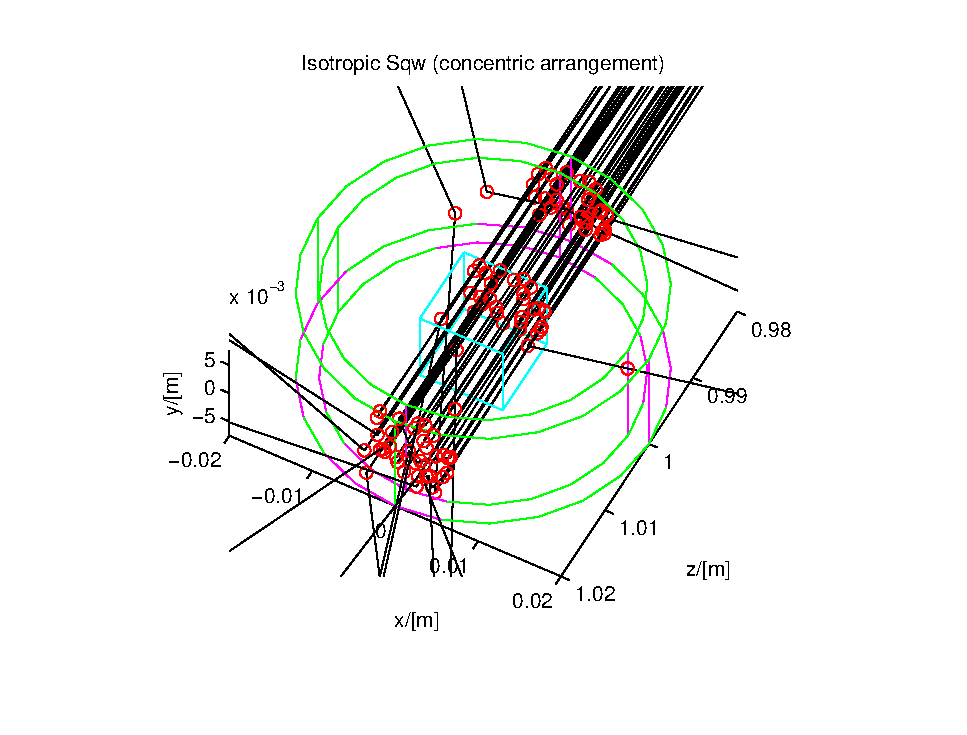
\includegraphics[width=0.9\textwidth]{figures/sqw.eps}
  \end{center}
\caption{An $l-^4$He sample in a cryostat, simulated with the Isotropic\_Sqw component in concentric geometry.}
\label{f:isotropic-sqw}
\end{figure}

The component assumes that the sample has the structure of an isotropic material. This stands for liquids, glasses (amorphous systems), polymers, gaz, and may be extended to powders. It simulates coherent and incoherent neutron scattering, and may be used to model isotropic samples, but also sample environments as concentric geometries are possible. The main input for the component is $S(q,\omega)$ tables, or powder structure files.

\subsection{Neutron interaction with matter}

When a neutron enters a material, according to usual models and letting the absorption aside to begin with, it 'sees' atoms as disks with a surface equal to the total scattering cross section of material $\sigma$. Each coherent and incoherent process is associated with a given probability to hit these cross-sections, according to $\sigma_{coh}$ or $\sigma_{inc}$. We may choose randomly a scattering position along the path, using e.g. an exponential decay probability. If the scattering condition is not satisfied, the neutron is transmitted, and leaves the sample. In any case, the absorption lowers the intensity according to an $e^{-\rho \sigma_{abs}d}$ absorption law along the propagation path $d$. In this process, the neutron is considered to be a particule.

Once the neutron 'knows' that something (terrible) is going to occur, it looks for a possible excitation to interact with. Then we turn to the wave description of the neutron, which interacts with the whole volume. The distribution of excitations, from which derives their relative intensity in the scattered beam, is simply the dynamic structre factor - or scattering law - $S(q,\omega)$. According to the definition of the density of states, we may use $g(\omega)$ as the probability law to scatter at a given energy transfer.

The neutron leaves the scattering point when a suitable $(q, \omega)$ choice has been found to satisfy the conservation laws. The process is iterated until the neutron leaves the volume of the material, eventually producing multiple scattering contributions.

The method shown below for multiple scattering handling is quite close in many respects to the earlier MSC \cite{msc}, Discus \cite{discus} and MSCAT \cite{mscat} programs, eventhough this implementation is original.

\subsection{Theoretical side}

\subsubsection{Pair correlation function $g(r)$ and Dynamic structure factor $S(q,\omega)$}

Following Squires (\cite{squires}, p63), the neutron differential scattering cross section for both coherent and incoherent processes is
\begin{equation}\label{eq:d2sigma}
\frac{d^2\sigma}{d\Omega dE_f} = \frac{\sigma}{4\pi}\frac{k_f}{k_i} N S(q, \omega)
\end{equation}
with usual notations: $N=\rho V$ is the number of atoms in the scattering volume $V$ with atomic number density $\rho$, $E_f, E_i, k_f, k_i$ are the energy and wavevectors of final and initial states respectively, $\sigma$ is the scattering cross-section, and $q,\omega$ are the wave-vector and energy transfer at the sample. The unit of the dynamical structure factor $S(q,\omega)$ is an inverse energy. We define its norm
\begin{equation}
|S| = \iint S(q,\omega) dq d\omega .
\end{equation}

Some easely measureable coherent quantities in a liquid are the \emph{static pair correlation function} $g(r)$ and the \emph{structure factor} $S(q)$, defined as:
\begin{eqnarray}
\rho g(\vec{r}) &=& \frac{1}{N} \sum_{i=1}^N \sum_{j \neq i} \langle \delta(\vec{r}+\vec{r}_i-\vec{r}_j) \rangle \\
S(\vec{q}) &=&\int S(\vec q,\omega) d\omega \label{eq:sq} \\
           &=&1 + \rho \int_V [g(\vec{r})-1] e^{i\vec{q}.\vec{r}} d\vec{r} \\
           &=&1 + \rho \int_{0}^{\infty} [g(r)-1] \frac{\sin(qr)}{qr} 4 \pi r^2 dr {\rm\ in\ isotropic\ materials.}
\end{eqnarray}
The latter expression, in isotropic materials, may be Fourier transformed as:
\begin{equation}
\label{eq:gr-sq}
g(r)-1 =\frac{1}{2\pi^2 \rho} \int_0^\infty q^2 [S(q) -1] \frac{sin(qr)}{qr} dq
\end{equation}
Both $g(r)$ and $S(q)$ converge to unity for large $r$ and $q$ values respectively, and they are representative of the atoms spatial distribution. In a liquid $\lim_{q \rightarrow 0} S(q) = \rho k_B T \chi_T$ where $\chi_T=(\frac{\partial \rho}{\partial P})_{V,T}$ is the compressibility \cite{Egelstaff67,fischer05}. In perfect gases, $S(q) = 1$ for all $q$. These quantities are obtained experimentaly from diffractometers.
In principle, $S_{inc}(q) = 1$, but a $q$ dependence is rather usual, partly due to the Debye-Waller factor $e^{-q^2 \langle u^2 \rangle}$. Anyway, $S(q)$ converges to unity at high $q$.

The static pair correlation function $g(r)$ is the probability to find a neighbouring atom at a given distance (unitless). Since $g(0) = 0$, Eq. (\ref{eq:gr-sq}) provides a useful normalization sum-rule for coherent $S(q)$:
\begin{equation}
\label{eq:sq-nomr1}
\int_0^\infty q^2 [S(q) - 1] dq = -2\pi^2\rho
\end{equation}
This means that the integrated oscilations (around 1) of $S_{coh}(q)$ are directly related to the density of the material $\rho$.
In practice, the function $S(q)$ is often known on a restricted range $q \in [0, q_{max} ]$, due to either limitations in the sample molecular dynamics simulation, or the measurement itself.
In first approximation we consider that Eq. (\ref{eq:sq-nomr1}) can be applied in this range, i.e. we neglect the large $q$ contributions providing $S(q)-1$ converges faster than $1/q^2$. Then, for any non-normalized coherent data set $S_{raw}$, we may obtain the normalized $S = \alpha S_{raw}$ with \cite{fischer05}
\begin{equation}
\label{eq:sq-nomr2}
\alpha \simeq \frac{q^3_{max}/3 - 2\pi^2 \rho}{\int_0^{q_{max}} q^2 S_{raw}(q) dq }
\end{equation}
This coherent normalization rule is only applied when parameter \verb+norm_sqw=-1+, which is recommanded for isotropic liquid-like materials. It is usually not suited for powders (see below).

We may measure, e.g. with time-of-flight instruments, the \emph{density of states} $g_{\omega}(\omega)$  which is the fraction of modes whose energy lie between $\omega$ and $\omega+d\omega$ \cite{lovesey84}
\begin{equation}
g_{\omega}(\omega) = \frac{\int S(q,\omega) dq}{|S|} .
\end{equation}
This function is normalized to unity, $\int g_{\omega}(\omega) d\omega = 1$ and is a probability distribution of mode energies in the material.

\subsubsection{Drawing probabilities from $S(q, \omega)$}

The main idea to implement the scattering from $S(q, \omega)$ is to basically make two consecutive Monte Carlo choices, applying the well known \emph{joint probability} theorem:
\begin{equation}
\label{eq:jointproba}
P(q \cap \omega) = P(\omega).P(q \mid \omega) .
\end{equation}

Thus we define $P(\omega)$ as the \emph{cumulated distribution} (primitive) of the density of states $g_{\omega}(\omega)$:
\begin{equation}\label{eq:Pw}
P(\omega) = \int_0^\omega g_{\omega}(\omega') d\omega'
\end{equation}
The function $P(\omega)$ is the probability for an excitation to have an energy lower than $\omega$.

Similarly, we define the conditional probability $P(q \mid \omega)$ to be, for each energy lying between $\omega$ and $\omega+d\omega$:
\begin{eqnarray}\label{eq:Pqw}
g_q(q\mid\omega) &=& \frac{S(q, \omega)}{\int S(q,\omega) dq} \\
P(q \mid \omega)    &=& \int_0^q g_q(q'\mid\omega) dq'
\end{eqnarray}
The former $g_q$ is the density of wavevector transfers for a selected energy transfer, and the latter $P(q \mid \omega)$ is the probability for an excitation to have a wavevector lower than $q$, for a given energy transfer $\omega$.

These probability distributions $g_\omega$ and $g_q$ implement importance sampling for scattering, 'directing' neutron events to high $S(q,\omega)$ regions.

\begin{figure}
  \begin{center}
    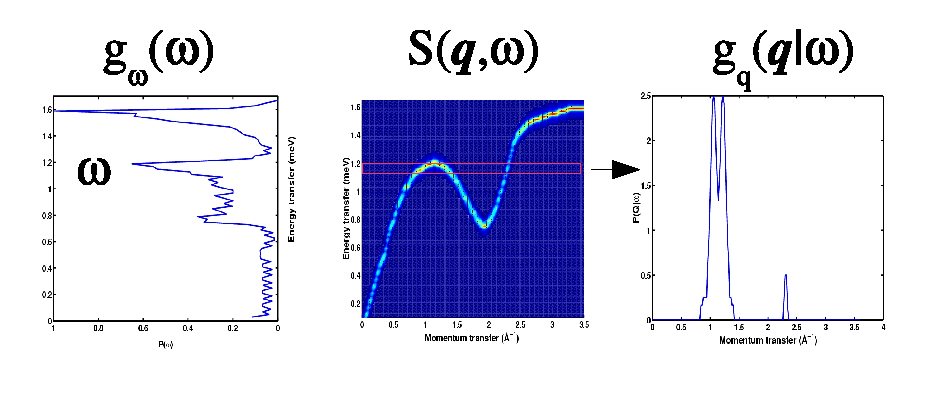
\includegraphics[width=0.9\textwidth]{figures/Sqw_sampling.eps}
  \end{center}
\caption{The probability functions extracted from $S(q,\omega)$. The energy transfer is first selected from the density of states $g_\omega$, then the wavevector is obtained from $g_q(\omega)$.}
\label{f:isotropic-sqw}
\end{figure}


\subsection{The method}

\subsubsection{Choosing the interaction type}

The method used is similar to the one adopted in the \verb+Single_crystal+ component (section \ref{s:Single_crystal}).

We first compute the absorption and total cross-section
\begin{eqnarray}
\sigma_{abs} &=& \sigma_{abs}^{{\rm 2200}}\frac{2200 m/s}{v} \\
\sigma_{tot} &=& \sigma_{abs} + \sigma_{coh} + \sigma_{inc}
\end{eqnarray}
as well as the neutron trajectory intersection with the geometry. This provides the total path length in the sample $d_{out}$ to the exit.
Defining the linear attenuation $\mu = \rho\sigma_{tot}$, the probability that the neutron scatters (or be absorbed) along path $d_{out}$ is $e^{-\mu d_{out}}$. If this condition is not satisfied, the neutron leaves the sample unchanged.
In the other case, we adjust the neutron weight by a factor
\begin{equation}
\pi_1 = \frac{\sigma_{coh} + \sigma_{inc}}{\sigma_{tot}}
\end{equation}
to account for the portion of absorbed neutrons along the path.
Additionally, we choose randomly the type of interaction with fractions $\sigma_{coh}$ and $\sigma_{inc}$.

\subsubsection{Choosing the interaction position}

If the straight path to the sample volume exit is $d_{out}$, the probability that the neutron scatters before exiting the sample at a distance $d_{scatt}$ is:
\begin{equation}
P(d_{scatt} < d_{out}) = \int_0^{d_{out}} \mu e^{-\mu x}dx = 1 - e^{-\mu d_{out}}. \\
\end{equation}
From that law, we may compute the cumulated distribution, which gives the probability for scattering to occur at a distance lower than $d_{scatt}$, knowing that the neutron interacts before $d_{out}$. This law may be analytically inverted so that the path length $d_{scatt}$ may be obtained directly from a uniform distribution random number $\xi$
\begin{equation}
d_{scatt} = -\frac{1}{\mu} \ln(1 - \xi[1 -e^{-\mu d_{out}}]).
\end{equation}
which then takes into account secondary extinction, originating from the decrease of the beam intensity through the sample (a kind of self shielding).
The Monte Carlo choice of the scattering position in the sample accounts for the $N \sigma$ factor in Eq. (\ref{eq:d2sigma}).

\subsubsection{Choosing the $q$ and $\omega$ transfer}

If no $S(q, \omega)$ data is available and the scattering process has been chosen as incoherent, we set $\omega=0$ and select randomly an outgoing wave vector $\boldsymbol{k}_f$.

In case the $S(q, \omega)$ data is available for the scattering process (coherent or incoherent), a random choice is made to select the energy transfert using $P(\omega)$ with the $g_\omega(\omega)$ probability distribution (Eq. \ref{eq:Pw}).
Similarly, we use $P(q \mid \omega)$ to select a wavevector transfer (Eq. \ref{eq:Pqw}).

Choosing a $(q, \omega)$ set and applying Eq. (\ref{eq:jointproba}), we have obtained a probabilistic normalized evaluation of the dynamical structure factor, which we multiply by the norm $|S|$ to obtain $S(q, \omega)$:
\begin{equation}
S(q, \omega) = |S|.g_\omega(\omega).g_q(q \mid \omega) .
\end{equation}
Then a selection between energy gain and loss is done with the detailed balance ratio $e^{-\hbar \omega / k_B T}$.

Finally, a statistical weightening by a factor:
\begin{equation}
\pi_2 = \frac{k_f}{k_i} |S|
\end{equation}
is required to account for Eq. (\ref{eq:d2sigma}). The factor $4 \pi$ in Eq. (\ref{eq:d2sigma}) originates from the integration of events over space, and is thus implicitely included in the Monte Carlo choice of the scattering direction.

\subsubsection{Choosing the scattered wave vector}

The next step is to check that conservation laws
\begin{eqnarray}
\hbar \omega &=& E_i - E_f = \frac{\hbar^2}{2m}(k_i^2 - k_f^2) \label{eq:q-transfert} \\
\vec q &=& \vec k_i - \vec k_f \label{eq:w-transfert}
\end{eqnarray}
can be satisfied. These conditions are closely related to the method for selecting the outgoing wave vector direction.

When the final wave vector has to be computed, the quantities $\vec{k}_i$, $\hbar \omega$ and $q = |\vec{q}|$ are known.
From the energy conservation law Eq. (\ref{eq:w-transfert}), we select ramdomly one of the two roots, $k_f^+$ and $k_f^-$.
The scattered wave vector is noted : $\vec{k}_f = k_f \vec{\hat k}_s$ where $\vec{\hat k}_s$ is a unit vector.\\
Since we only know the norm of the scattering vector $\vec{q}$, the momentum conservation law Eq. (\ref{eq:q-transfert}) may be expressed as
\begin{align}
q^2 = |\vec{k}_i -\vec{k}_f|^2 = |k_i^2 + k_f^2 - 2 k_f \vec{k}_i \cdot \vec{\hat k}_s
\end{align}
where $\vec{k}_i \cdot \vec{\hat k}_s$ stands for the dot product of the vectors.\\
Now, we should solve :
\begin{align}
\vec{k}_i \cdot \vec{\hat k}_s &= \frac{1}{2k_f} (k_i^2 + k_f^2 - q^2) = C \\
|\vec{\hat k}_s| &= 1
\end{align}
where $C$ is a constant.
$\vec{\hat k}_s$ can be decomposed as : $\vec{\hat k}_s = B \vec{k}_i + \vec{u}_0$ where $B$ is a constant and $\vec{u}_0$ is a vector of $Vect(\vec{k}_i)^{\bot}$ (that is the orthogonal of the space generated by $\vec{k}_i$), which is a plane $P$.
Since we have : $\vec{k}_i \cdot \vec{\hat k}_s = C$, we may write : $B = \frac{C}{k_i^2}$.
\begin{figure}[!h]
\begin{center}
\includegraphics*[height=6cm]{figures/calckf_2.eps}
\caption{How to compute the outgoing wavevector direction $\vec{\hat k}_s$}
\label{fig:ann_kf}
\end{center}
\end{figure}
The vectors $\vec{u}_0$ such that $|\vec{\hat k}_s| = 1$ define a circle of radius $R$ : $|\vec{u}_0|~=~R$.
Since $\vec{u}_0$ and $B \vec{k}_i$ are orthogonal, we find :
\begin{align}
\frac{C^2}{k_i^2} + R^2 = |\vec{\hat k}_s|^2 = 1
\end{align}
from which we deduce the radius of the circle :
\begin{align}
R = \sqrt{1 - \frac{C^2}{k_i^2}}.
\end{align}
Let us now define an orthonormal basis ($\vec{u}_1,\vec{u}_2$) of the plane containing $\vec{u}_0$.
$\vec{u}_0$ can be decomposed as : $\vec{u}_0~=~R(\cos \theta \vec{u}_1 + \sin \theta \vec{u}_2)$, where $\theta$ can be randomly drawn for a uniform distribution.
Finally, we obtain :
\begin{align}
\vec{\hat k}_s = \frac{C^2}{k_i^2} \vec{k}_i + R (\cos \theta \vec{u}_1 + \sin \theta \vec{u}_2)
\end{align}

\subsubsection{Extension to powder elastic scattering}

In principle, the component can work in purely elastic mode if only the $\omega = 0$ column is available in $S$.
Anyway, in the diffractionists world, people do not usually define scattering with $S(q)$ (Eq. \ref{eq:sq}), but through the scattering vector $\boldsymbol{\tau}$, multiplicity $z(\tau)$ (for powders), and $|F^2|$ structure factors including Debye-Waller factors, as in Eq. \ref{eq:sigma_coh_el}.

When doing diffraction, and neglecting inelastic contribution as first approximation, we may integrate Eq. \ref{eq:d2sigma}, keeping $k_i = k_f$.
\begin{eqnarray}
\left(\frac{d\sigma}{d\Omega}\right)_{\rm coh.el.}(|q|) &=& \int_0^\infty \frac{d^2\sigma_{coh}}{d\Omega dE_f} dE_f = \frac{N \sigma_{coh}}{4\pi} S_{coh}(q) \\
& = & N\frac{(2\pi)^3}{V_0}\sum_{\boldsymbol{\tau}} \delta(\boldsymbol{\tau} - \boldsymbol{q})|F_{\boldsymbol{\tau}}|^2 {\rm\ from\ Eq.\ (\ref{eq:sigma_coh_el})}
\end{eqnarray}
with $V_0 = 1/\rho$ being the volume of a lattice unit cell. Then we come to the formal equivalence, in the powder case \cite{squires} (integration over Debye-Scherrer cones):
\begin{eqnarray}\label{eq:sq-F2}
S_{coh}(q) = \frac{4 \pi \rho}{\sigma_{coh}} \frac{z(q)}{q} |F_q|^2 {\rm\ in\ a\ powder.}
\end{eqnarray}
for each lattice Bragg peak wave vector $q$.
The normalization rule Eq. (\ref{eq:sq-nomr2}) can not usually be applied for powders, as the $S(q)$ is a set of Dirac peaks for which the $\int q^2 S(q) dq$ is difficult to compute, and $S(q)$ does not converge to unity for large $q$.

Of course, the component PowderN (see section \ref{powder}) can handle powder samples more efficiently (faster, better accuracy), but does not take into account multiple scattering.

\subsubsection{Important remarks and limitations}

Since the choice of the interaction type, we know that the neutron \emph{must} scatter, with an appropriate $\vec k_f$ outgoing wave vector. If any of the choices in the method fails:
\begin{enumerate}
\item the roots $k_f^+$ and $k_f^-$ are imaginary, which means that conservation laws can not be satisfied and for instance the selected energy transfert is higher than the incoming neutron energy
\item the radius of the target circle $R$ is imaginary
\end{enumerate}
then a new $(q, \omega)$ set is drawn, and the process is iterated until sucess or - at last - removal of the neutron event. This latter absorption is then reported at the end of the simulation, as it never occurs in reality - neutrons that scatter do find a suitable $(q, \omega)$ set.\index{Removed neutron events}

A way to avoid this is to focus the $q,\omega$ range from the $S(q, \omega)$ data file to the actual beam characteristics (matching instrument dynamical range). This is done e.g. by setting the component parameter $wmax$ to the maximum energy of the incoming beam. In a few words, the $S(q,\omega)$ data set extension in $Q$ and $\omega$ should preferably be smaller than the extension of the incoming beam and the scattered beam of interest for the experiment. Otherwise some Monte carlo choices lead to scattering in non useful regions of $S$, which reduces dramatically the algorithm efficiency, possibly removing neutrons by underestimating intensity.\index{Bugs} An automatic probability table optimization may be activated when setting parameter \verb+auto_qw=1+. This is higly recommanded, but may sometimes miss a few neutrons if the $q,\omega$ beam range has been guessed too small.

Focusing the $q$ and $\omega$ range, to the one being able to scatter the incoming beam, when using the component does improve significantly the speed of the computation. Additionally, if you restrict the scattering the first order only (parameter order=1), then you may specify the angular vertical extension $d\phi$ of the scattering area to gain optimized focusing. This option does not apply when handling multiple scattering (which emits in $4\pi$ many times before exiting the sample).

A bilinear interpolation for the $Q,\omega$ determination is recommanded to improve the accuracy of the scattered intensity, but it may be unactivated when setting parameter \verb+interpolate=0+. This will often result in a discrete $Q,\omega$ sampling.

As indicated in the previous section, the Isotropic\_Sqw component is not as accurate as PowderN for powders scattering for single scattering.

\subsection{The implementation}

\begin{table}
  \begin{center}
  {\let\my=\\
    \begin{tabular}{|lr|p{0.6\textwidth}|}
    \hline
Parameter & type & meaning \\
    \hline
Sqw\_coh   & string              & Coherent scattering data file name. Use 0 or "" to disable  \\
Sqw\_inc   & string              & Incoherent scattering data file name. Use 0 or "" to scatter isotropically (Vanadium like)  \\
sigma\_coh & [barns]      & Coherent scattering cross-section. 0 to disable \\
sigma\_inc & [barns]      & Incoherent scattering cross-section. 0 to disable \\
sigma\_abs & [barns]      & Absorption cross-section. 0 to disable  \\
V\_rho     & [\AA$^{-3}$] & atomic number density. May also be specified with molar weight \emph{weight} in [g/mol] and material \emph{density} in [g/cm$^3$] \\
T          & [K]          & Temperature. 0 disables detailed balance \\
    \hline
xwidth   & [m] & \\
yheight  & [m] & dimensions of a box shaped geometry \\
zthick   & [m] & \\
radius\_o & [m] & dimensions of a cylinder shaped geometry  \\
radius\_i & [m] & sphere geometry if radius\_i=0  \\
thickness& [m] & thickness of hollow shape  \\
    \hline
norm\_sqw & number  & When positive, the value is used as the integral of S(q,w). Null value uses computed integral. Any negative value will normalize on the density (for liquids, NOT recommanded for Powders) \\
auto\_qw  & boolean & Automatically optimize probability tables during simulation (recommanded)  \\
interpolate & boolean & Smooth $S(q,\omega)$ table (recommanded) \\
order     & integer & Limit multiple scattering up to given order. 0 means no limitations  \\
concentric& boolean & Enables to 'enter' inside concentric hollow geometries  \\
    \hline
    \end{tabular}
    \caption{Main Isotropic\_Sqw component parameters}
    \label{t:sqw-param}
  }
  \end{center}
\end{table}

\subsubsection{Geometry}

The geometry for the component may be box, cylinder and sphere shaped, either filled or hollow. Relevant parameters for this purpose are as follow:
\begin{itemize}
\item {\bf box}: dimensions are $x_{width} \times y_{height} \times z_{thick}$.
\item {\bf box, hollow}: \emph{idem}, and the side wall thickness is set with $thickness$.
\item {\bf cylinder}: dimensions are $r_o$ for the radius and $y_{height}$ for the heigh.
\item {\bf cylinder, hollow}: \emph{idem}, and hollow part is set with either $r_i$ internal radius, or $thickness$.
\item {\bf sphere}: dimension is $r_o$ for the radius.
\item {\bf sphere, hollow}: \emph{idem}, and hollow part is set with either $r_i$ internal radius, or $thickness$.
\end{itemize}
The AT position corresponds to the center of the sample.

Hollow shapes are particularly useful to model complex sample environments. Refer to section below for more details on this topic.

\subsubsection{Dynamical structure factor}

The material behaviour is specified through the total scattering cross-sections $\sigma_{coh}$, $\sigma_{inc}$, $\sigma_{abs}$, and the $S(q, \omega)$ data files.

If you are lucky enough to have access to separated coherent and incoherent contributions (e.g. from material simulation), simply set Sqw\_coh and Sqw\_inc paremeter to the files names. If on the other hand you have access to a global data set containing incoherent scattering as well (e.g. the result of a previous experiment), use Sqw\_coh parameter, set the $\sigma_{coh}$ parameter to the sum of both contributions $\sigma_{coh}+\sigma_{inc}$, and set $\sigma_{inc}=0$. This way we only use one of the two implemented  scattering channels. Such global data sets may originate from previous experiments, as far as you have applied all known corrections (multiple scattering, geometry, ...).

In any case, the accuracy of the $S(q, \omega)$ data limits the $Q$ and $\omega$ resolution of the simulation, eventhough a bilinear interpolation is performed in order to smooth a too coarse binning. The sampling of data files should then be as thin as possible.

If the Sqw\_inc parameter is left unset but the $\sigma_{inc}$ is \emph{not} zero, an isotropic incoherent elastic scattering is used, just like the V\_sample component (see section \ref{s:v_sample}).

Anyway, as explained below, it is also possible to only simulate the elastic scattering from a powder file (see below). Moreover, as there are two process channels (coherent and incoherent), it is possible to simulate a mixture of two powders, with fractions proportional to $\sigma_{coh}$ and $\sigma_{inc}$.

\subsubsection{File formats: $S(q,\omega)$ inelastic scattering}

The format of the data files is free text, consisting of three numerical block, separated by empty lines or comments, in the following order
\begin{enumerate}
\item A vector of length $m$ containing wavevector $q$ values, in \AA$^{-1}$.
\item A vector of length $n$ containing energy $\omega$ values, in meV.
\item A matrix of size $m$ rows by $n$ columns, of $S(q, \omega)$ values, in meV$^{-1}$.
\end{enumerate}
Any line beginning with any character of \verb+#;/%+ is considered to be a comment, and lines which can not be read as vectors/matrices are ignored.
Example files are listed as \verb+*.sqw+ files in directory \verb+MCSTAS/data+.

The file header may optionally contain parameter settings for the material, as comments, with keywords as is the following example:
\begin{verbatim}
  #V_0         0.07
  #sigma_abs   5
  #sigma_inc   4.8
  #sigma_coh   1
  #Temperature 10
\end{verbatim}
Some \verb+sqw+ data files are included in the \MCS\ distribution data directory, and they contain material parameter settings in their header, so that you may use:
\begin{verbatim}
Isotropic_Sqw(<geometry parameters>, Sqw_coh="He4.sqw", T=10)
\end{verbatim}

\subsubsection{File formats: $S(q)$ liquids}

This file format provides a mean to import directly an $S(q)$ data set, when setting parameters:
\begin{verbatim}
  powder_format=qSq
\end{verbatim}
The 'Sqw\_coh' (or 'Sqw\_inc') file should contains a single numerical block, which column assignment is defaulted as $q$ and $S(q)$ being the first and second columns respectively. This may be overridden from the file header with '\#column' keywords, as in the example:
\begin{verbatim}
  #column_q  2
  #column_Sq 1
\end{verbatim}
Such files can only handle elastic scattering.

\subsubsection{File formats: powder structures (LAZY, Fullprof, Crystallographica)}

Data files as used by the component PowderN may also be read. Data files of type \verb'lau' and \verb'laz' in the \MCS\ distribution data directory are self-documented in their header. They do not need any additional parameters to be used, as in the example:
\begin{verbatim}
  Isotropic_Sqw(<geometry parameters>, Sqw_coh="Al.laz")
\end{verbatim}
Other column-based file formats may also be imported e.g. with parameters such as:
\begin{verbatim}
  powder_format=Crystallographica
  powder_format=Fullprof
  powder_Dd    =0
  powder_DW    =1
\end{verbatim}
The last two parameters may as well be specified in the data file header with lines:
\begin{verbatim}
  #Debye_Waller 1
  #Delta_d/d    1e-3
\end{verbatim}
The powder description is then translated into $S(q)$ by using Eq. (\ref{eq:sq-F2}).
In this case, the density $\rho = n/V_0$ is the number of atoms in the inverse volume of the unit cell.

As the component builds an $S(q)$ from the powder structure description, the accuracy of the Isotropic\_Sqw component is limited by the binning during that conversion. This is usually enough to describe sample environments including powders (aluminium, copper, ...), but it is recommanded to rather use PowderN for faster and accurate powder diffraction, eventthough this latter does not implement multiple scattering.

Such files can only handle elastic scattering. A list of common powder definition files is available in Table \ref{t:powders-data} (page \pageref{t:powders-data}).

\subsubsection{Concentric geometries, sample environment}
\index{Sample environments}

The component has been designed in a way which enables to describe complex imbricated set-ups, i.e. what you need to simulate sample environments. To do so, one has first to use hollow shapes, they keep in mind that each surrounding geometry should be first declared before the central position (usially the sample) with the \verb+concentric=1+ parameter, but also duplicated (with an other instance name) at a symetric position with regards to the centre as in the example (shown in Fig. \ref{f:isotropic-sqw}):
\begin{verbatim}
COMPONENT s_in=Isotropic_Sqw(
  thickness=0.001, radius_o=0.02, yheight=0.015,
  Sqw_coh="Al.laz", concentric=1)
AT (0,0,1) RELATIVE a

COMPONENT sample=Isotropic_Sqw(
  xwidth=0.01, yheight=0.01, zthick=0.01,
  Sqw_coh="He4_coh.sqw")
AT (0,0,1) RELATIVE a

COMPONENT s_out=Isotropic_Sqw(
  thickness=0.001, radius_o=0.02, yheight=0.015,
  Sqw_coh="Al.laz")
AT (0,0,1) RELATIVE a
\end{verbatim}
Central component may be of any type, not specifically an Isotropic\_Sqw instance. It could be for instance a Single\_crystal or a PowderN.
In principle, the number of surrounding shells is not restricted.
The only restriction is that neutrons that scatter (in $4\pi$) can not come back in the instrument description, so that some of the multiple scattering events are lost. Namely, in the previous example, neutrons scattered by the outer wall of the cryostat \verb+s_out+ can not come back to the sample or to the other cryostat wall \verb+s_in+. As these neutrons have usually few chances to reach the rest of the simulation, we expect that the approximation is fair.

\subsection{Validation}
For Vanadium incoherent scattering mode, V\_sample, PowderN, Single\_crystal and Isotropic\_Sqw produce equivalent results, eventhough the two later are more accurate (geometry, multiple scattering). Execution times are equivalent.

Compared to the PowderN component, the $S(q)$ method is twice slower in computation time (but often brings more statistics), and intensity is usually lower by a factor 1 to 2. The PowderN component is intrinsically more accurate as each Bragg peak is handled separately as an exact Dirac peak, with optional $\Delta q$ spreading. In Isotropic\_Sqw, an approximated $S(q)$ table is built from the $F^2$ data, and is coarser.



